\documentclass[14pt,a4paper]{extarticle}
\usepackage{fontspec}
\setmainfont{Times New Roman}
\usepackage[english,russian]{babel}
\usepackage{graphicx} % Required for inserting images
\usepackage[top=20mm,bottom=20mm,left=30mm,right=15mm]{geometry}
\usepackage{xcolor}
\usepackage{setspace}
\usepackage{tabularx}
\usepackage{fancyhdr}
\usepackage{caption}
\usepackage{graphicx}
\usepackage{placeins}
\usepackage{caption}
\usepackage{subcaption}
\usepackage{amsmath}
\usepackage{float}

\setlength{\parindent}{15mm}
\setstretch{1.5}
\linespread{1.25}
\tolerance=1
\emergencystretch=\maxdimen
\hyphenpenalty=10000
\exhyphenpenalty=10000
\usepackage{titlesec}
\titleformat{\section}[hang]{\normalfont\bfseries}{\thesection}{}{}
\titlespacing{\section}{15mm}{0pt}{0pt}
\captionsetup[figure]{name = {Рисунок}, labelsep = endash}

\begin{document}
\begin{titlepage}
    \begin{center}
    {\bfseries
    МИНОБРНАУКИ РОССИИ \\ САНКТ-ПЕТЕРБУРГСКИЙ ГОСУДАРСТВЕННЫЙ \\ ЭЛЕКТРОТЕХНИЧЕСКИЙ УНИВЕРСИТЕТ \\ <<ЛЭТИ>> ИМ. В.И. УЛЬЯНОВА (ЛЕНИНА)\\Кафедра САПР \vspace{0.23\textheight}
    
    ОТЧЕТ \\ по практической работе №6 \\ по дисциплине <<Информационные технологии>> \\ Тема: Частные производные функции нескольких переменных. \\
    \vspace{0.28\textheight}
        }
        \begin{table}[h!]
            \begin{tabularx}{\textwidth}{p{60mm}X>{\centering\arraybackslash}p{45mm}}
                Студент гр. 4352 & \_\_\_\_\_\_\_\_\_\_\_\_\_\_\_\_\_\_\_\_ & {Колесникова М. А.} \\ [5.4mm]  
                Преподаватель    & \_\_\_\_\_\_\_\_\_\_\_\_\_\_\_\_\_\_\_\_ & {Копец Е. Е.} \\ [5.4mm]
            \end{tabularx}
        \end{table}
    Санкт-Петербург\par
        2025
    \end{center}
\end{titlepage}
\setcounter{page}{2}

\section*{Цель работы.}

Научиться находить частные производные для функций с несколькими переменными и сравнивать их.

\section*{Основные теоретические положения.}

Чтобы вычислить среднее квадратичное для функций нужно взять каждую пару значений $(x_1,x_2)$
из списка объектов и подставить их в функцию с помощью subs. Затем для каждого объекта вычисляется
разность между предсказанным значением и целевым значением, эта разность возводится в квадрат.
Все квадраты ошибок складываются и делятся на их количество (рис. \ref{pic:cod}).

\begin{figure}[h!]
    \centering
    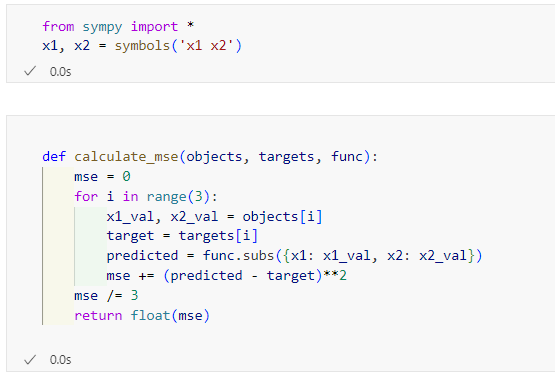
\includegraphics[scale=0.7]{pic6/1.png}
    \caption{Код для нахождения MSE}
    \label{pic:cod}
\end{figure}
\FloatBarrier

В первом наборе данных функция
$f_1=-2x_2+x_1-7$ имеет значение MSE, чем функция $f_2=20x_2+3x_1-4$ (рис. \ref{pic:mse1}).

\begin{figure}[h!]
    \centering
    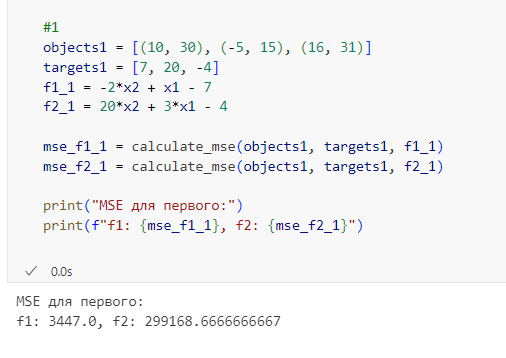
\includegraphics[scale=0.9]{pic6/1.1.png}
    \caption{MSE для первого набора}
    \label{pic:mse1}
\end{figure}
\FloatBarrier

В первом наборе данных функция
$f_1=-2x_2-x_1+60$ имеет значение MSE, чем функция $f_2=2x_2+17x_1-9$ (рис. \ref{pic:mse2}).

\begin{figure}[h!]
    \centering
    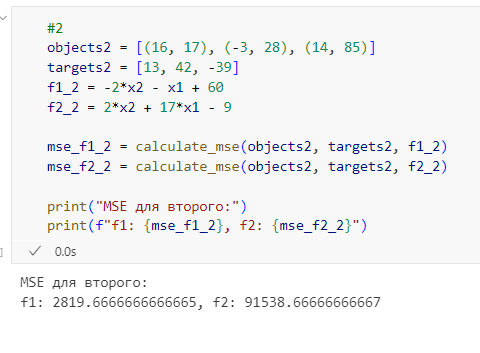
\includegraphics[scale=0.9]{pic6/1.2.png}
    \caption{MSE для второго набора}
    \label{pic:mse2}
\end{figure}
\FloatBarrier

В первом наборе данных функция
$f_1=-4x_2+7x_1-11$ имеет значение MSE, чем функция $f_2=-0.5x_2+9x_1-400$ (рис. \ref{pic:mse3}).

\begin{figure}[h!]
    \centering
    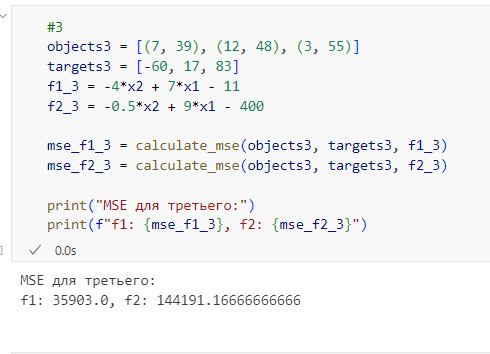
\includegraphics[scale=0.9]{pic6/1.3.png}
    \caption{MSE для третьего набора}
    \label{pic:mse3}
\end{figure}
\FloatBarrier

Нахождение частные производных:


\begin{enumerate}
    \item 
    \[
    f(x_1, x_2) = 10x_1 - 5x_2
    \]
    \[
    \frac{\partial f}{\partial x_1} = 10 - 0 = 10
    \]
    \[
    \frac{\partial f}{\partial x_2} = 0 - 5 = -5
    \]

    \item 
    \[
    f(x_1, x_2) = 3x_1 + 4x_2 + 7
    \]
    \[
    \frac{\partial f}{\partial x_1} = 3 + 0 + 0 = 3
    \]
    \[
    \frac{\partial f}{\partial x_2} = 0 + 4 + 0 = 4
    \]

    \item 
    \[
    f(x_1, x_2) = x_1^2
    \]
    \[
    \frac{\partial f}{\partial x_1} = 2x_1
    \]
    \[
    \frac{\partial f}{\partial x_2} = 0
    \]

    \item 
    \[
    f(x_1, x_2, x_3) = x_1 + 5x_2 - 6x_3 + 3
    \]
    \[
    \frac{\partial f}{\partial x_1} = 1 + 0 + 0 + 0 = 1
    \]
    \[
    \frac{\partial f}{\partial x_2} = 0 + 5 + 0 + 0 = 5
    \]
    \[
    \frac{\partial f}{\partial x_3} = 0 - 6 + 0 + 0 = -6
    \]

    \item 
    \[
    f(x_1, x_2, x_3) = 10x_1 - x_1^2 + 4x_1^3
    \]
    \[
    \frac{\partial f}{\partial x_1} = 10 - 2x_1 + 12x_1^2
    \]
    \[
    \frac{\partial f}{\partial x_2} = 0
    \]
    \[
    \frac{\partial f}{\partial x_3} = 0
    \]

    \item 
    \[
    f(x_1, x_2, x_3) = x_1^2 + 12x_1x_2 + 4x_2^3 + x_3
    \]
    \[
    \frac{\partial f}{\partial x_1} = 2x_1 + 12x_2
    \]
    \[
    \frac{\partial f}{\partial x_2} = 12x_1 + 12x_2^2
    \]
    \[
    \frac{\partial f}{\partial x_3} = 1
    \]
\end{enumerate}

Частные производные среднеквадратичной ошибки можно найти с помощью sympy (рис. \ref{pic:mse}).

\begin{figure}[h!]
    \centering
    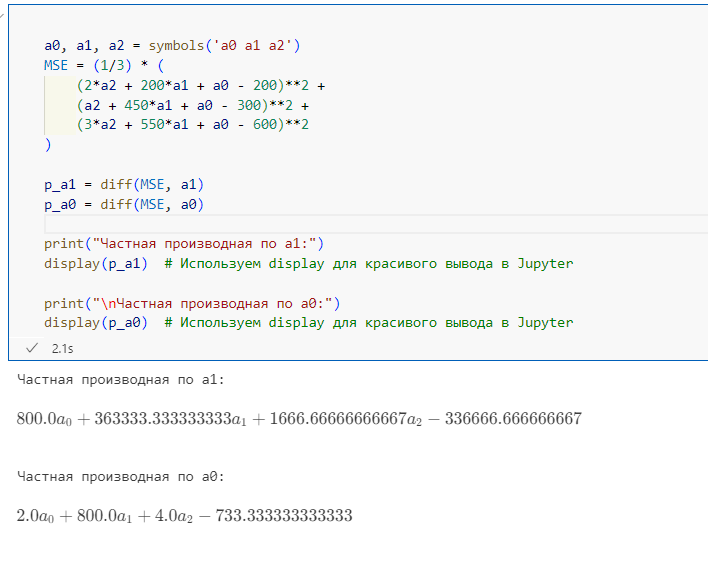
\includegraphics[scale=0.9]{pic6/3.png}
    \caption{Производные MSE по $a_0$ и $a_1$}
    \label{pic:mse}
\end{figure}
\FloatBarrier

Функция среднеквадратичной ошибки для четвёртого задания задаётся как:
\[
\text{MSE} = \frac{1}{3} \sum_{i=1}^3 \left( \text{Площадь}_i - (a_0 + a_1 \cdot \text{Цена}_i + a_2 \cdot \text{Этажи}_i) \right)^2,
\]
Частные производные MSE по коэффициентам $a_0$, $a_1$ и $a_2$:
\[
\frac{\partial \text{MSE}}{\partial a_0} = -\frac{2}{3} \sum_{i=1}^3 \left( \text{Площадь}_i - (a_0 + a_1 \cdot \text{Цена}_i + a_2 \cdot \text{Этажи}_i) \right),
\]
\[
\frac{\partial \text{MSE}}{\partial a_1} = -\frac{2}{3} \sum_{i=1}^3 \left( \text{Площадь}_i - (a_0 + a_1 \cdot \text{Цена}_i + a_2 \cdot \text{Этажи}_i) \right) \cdot \text{Цена}_i,
\]
\[
\frac{\partial \text{MSE}}{\partial a_2} = -\frac{2}{3} \sum_{i=1}^3 \left( \text{Площадь}_i - (a_0 + a_1 \cdot \text{Цена}_i + a_2 \cdot \text{Этажи}_i) \right) \cdot \text{Этажи}_i.
\]

Далее с помощью библиотеки sympy можно найти все необходимые
производные и предсказать площадь дома,
в этом случае точкой минимума являются найденные коэффициенты (рис. \ref{pic:house}).

\begin{figure}[h!]
    \centering
    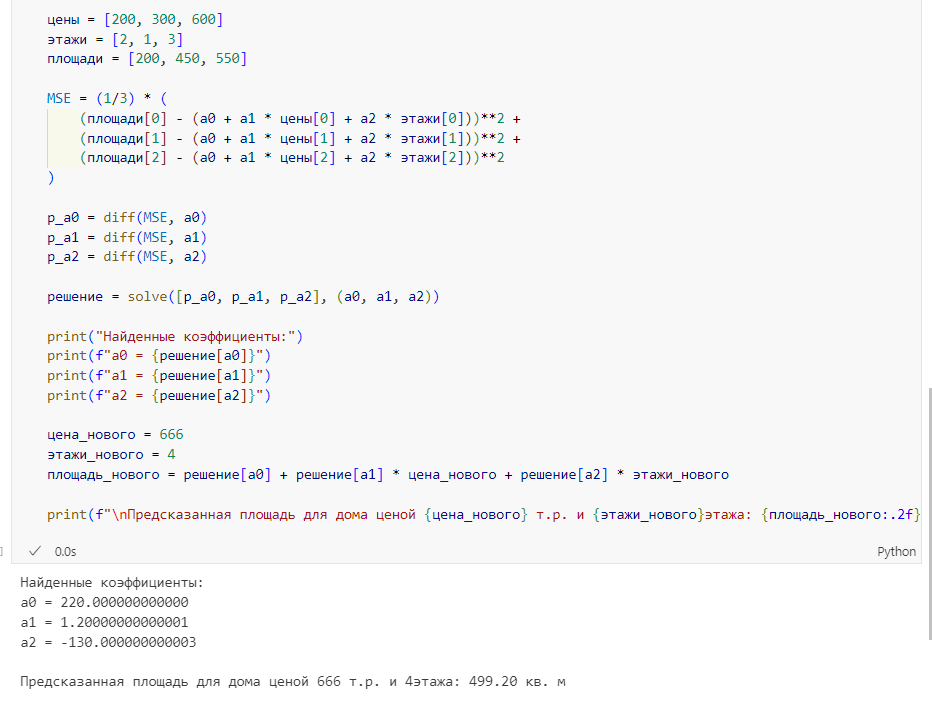
\includegraphics[scale=0.66]{pic6/4.png}
    \caption{Предсказание цены дома}
    \label{pic:house}
\end{figure}
\FloatBarrier

\section*{Вывод.}

В ходе работы были изучены частные производные функции нескольких переменных.
Также были найдены их значения и была проведена работа по сравнению MSE
различных функций-кандидатов.

\end{document}